% \documentclass[aspectratio=169,notes]{beamer}
\documentclass[aspectratio=169]{beamer}
\usetheme[faculty=phil]{fibeamer}
\usepackage{polyglossia}
\setmainlanguage{english} %% main locale instead of `english`, you
%% can typeset the presentation in either Czech or Slovak,
%% respectively.
\setotherlanguages{russian} %% The additional keys allow
%%
%%   \begin{otherlanguage}{czech}   ... \end{otherlanguage}
%%   \begin{otherlanguage}{slovak}  ... \end{otherlanguage}
%%
%% These macros specify information about the presentation
\title[AGLA2]{Analytical Geometry and Linear Algebra II, Lab 12} %% that will be typeset on the
\subtitle{Similar matrices \\ Singular value decomposition - SVD \\ Left and right inverses. Pseudoinverse
         } %% title page.
\author{Oleg Bulichev}
%% These additional packages are used within the document:
\usepackage{ragged2e}  % `\justifying` text
\usepackage{booktabs}  % Tables
\usepackage{tabularx}
\usepackage{tikz}      % Diagrams
\usetikzlibrary{calc, shapes, backgrounds}
\usepackage{amsmath, amssymb}
\usepackage{url}       % `\url`s
\usepackage{listings}  % Code listings
% \usepackage{subfigure}
\usepackage{floatrow}
\usepackage{subcaption}
\usepackage{mathtools}
\usepackage{todonotes}
\usepackage{fontspec}
\usepackage{multicol}
\usepackage{pdfpages}
\usepackage{wrapfig}
\usepackage{animate}
\usepackage{booktabs}
\usepackage{multirow}

\graphicspath{{resources/}}
\frenchspacing

\setbeamertemplate{caption}[numbered]
\usetikzlibrary{graphs}

% \usepackage[backend=biber,style=ieee,autocite=footnote]{biblatex}
% \addbibresource{biblio.bib}
% \DefineBibliographyStrings{english}{%
%   bibliography = {References},}

\newcommand{\oleg}[2][] {\todo[color=red, #1] {OLEG:\\ #2}}
\newcommand{\fbckg}[1]{\usebackgroundtemplate{\includegraphics[width=\paperwidth]{#1}}}%frame background

\usepackage[framemethod=TikZ]{mdframed}
\newcommand{\dbox}[1]{
\begin{mdframed}[roundcorner=3pt, backgroundcolor=yellow, linewidth=0]
\vspace{1mm}
{#1}
\vspace{1mm}
\end{mdframed}
}

\begin{document}
\setlength{\abovedisplayskip}{0pt}
\setlength{\belowdisplayskip}{0pt}
\setlength{\abovedisplayshortskip}{0pt}
\setlength{\belowdisplayshortskip}{0pt}

\fbckg{fibeamer/figs/title_page.png}
\frame[c]{\setcounter{framenumber}{0}
    \usebeamerfont{title}%
    \usebeamercolor[fg]{title}%
    \begin{minipage}[b][6.5\baselineskip][b]{\textwidth}%
        \textcolor{black}{\raggedright\inserttitle}
    \end{minipage}
    % \vskip-1.5\baselineskip

    \usebeamerfont{subtitle}%
    \usebeamercolor[fg]{framesubtitle}%
    \begin{minipage}[b][3\baselineskip][b]{\textwidth}
        \raggedright%
        \insertsubtitle%
    \end{minipage}
    \vskip.25\baselineskip
}
%   \frame[c]{\maketitle}

\fbckg{fibeamer/figs/common.png}

\begin{frame}[c]{How I spent last weekend}
    \framesubtitle{}
    \begin{figure}[H]
        \begin{subfigure}{0.64\textwidth}
            \centering
\includegraphics[height=5.5cm,width=1\textwidth,keepaspectratio]{jobless_reincarnation.jpg}
            \caption*{Jobless Reincarnation ranobe: $4342/6859$ pages. Tome 19th}
        \end{subfigure}     
        \hfill
        \begin{subfigure}{0.34\textwidth}
            \centering\includegraphics[height=5.5cm,width=1\textwidth,keepaspectratio]{catamaran.jpg}
            \caption*{Catamaran sailing training with KFU}
        \end{subfigure}
    \end{figure}
\end{frame}

\begin{frame}[t]{Similar Matrices}
\framesubtitle{}
    \LARGE
    \centering
    All the matrices $A=BCB^{-1}$ are "similar". They all share the eigenvalues of $C$. \\
    \begin{example}
        \Large
        $A = \begin{bmatrix}
        2 & 1\\ 
        1 & 2 
        \end{bmatrix} \rightarrow \lambda =3,\ 1;$  $S^{-1}AS=\Lambda_{A} = \begin{bmatrix}
        3 & 0\\ 
        0 & 1 
        \end{bmatrix}$, $S$ -- eigenvectors \\ 
        \vspace{-0.4cm}
        Let's find other similar matrix: $M^{-1}AM=T$, $M=\begin{bmatrix}
        1 & 4\\ 
        0 & 1 
        \end{bmatrix}$, $M$ is \\ 
        \vspace{-0.4cm}
        random matrix. $T = \begin{bmatrix}
        -2 & -15\\ 
        1 & 6 
        \end{bmatrix}$, which $\lambda$ are also $3,\ 1$.
    \end{example}
\end{frame}

\begin{frame}[t]{Similar Matrices}
\framesubtitle{Properties}
Because matrices are similar if and only if they represent the \textit{same linear operator with respect to (possibly) different bases}, similar matrices share all properties of their shared underlying operator:
\begin{itemize}
    \item Rank
    \item Characteristic polynomial, and attributes that can be derived from it: \begin{itemize}
        \item Eigenvalues
        \item Determinant
        \item Trace
    \end{itemize}
\end{itemize}

\href{https://en.wikipedia.org/wiki/Matrix_similarity}{More info} can be found here. This topic was used for checking understanding LA by the students (\href{https://www.tandfonline.com/doi/full/10.1080/07380569.2018.1491774}{paper}).

\end{frame}

\begin{frame}[c]{The primary goal of SVD}
\framesubtitle{}
\centering\LARGE
To “X-RAY” matrix

(To understand the structure of matrix)
\end{frame}

\begin{frame}[t]{Singular Value Decomposition (SVD)}
\framesubtitle{3 ways of explanation}
    \begin{columns}[T,onlytextwidth]
        \begin{column}{0.69\textwidth}
            \begin{enumerate}
                \item Linear transformation – \href{https://youtu.be/EokL7E6o1AE}{Kutz video}
                \item Algebraic – \href{https://www.youtube.com/watch?v=rYz83XPxiZo&list=PLUl4u3cNGP63oMNUHXqIUcrkS2PivhN3k&index=8}{MIT video (Strang)}, \href{https://youtu.be/EfZsEFhHcNM}{Aaron Greiner video}
                \item As a tool for DS  – \href{https://youtu.be/P5mlg91as1c}{Stanford video}, \href{https://youtu.be/yA66KsFqUAE}{Brunton video}
            \end{enumerate}

            According to Kholodov words, SVD was created for \textit{finding an inverse for any matrices}. It is needed in linear transformation related operations. Other properties were found afterwards. 
        \end{column}
        \begin{column}{0.29\textwidth}
            \vspace{-1cm}
            \begin{figure}[H]
                \centering
\includegraphics[height=6cm,width=1\textwidth,keepaspectratio]{two_buttons.jpg}
                % \caption{caption_name}
                \label{fig:two_buttons.jpg}
            \end{figure}
        \end{column}
    \end{columns}
\end{frame}

\note{
    В чем крутость СВД:
    \begin{itemize}
        \item Он создан для работы с большими данными
        \item Революция. По мнению Брунтона, это второе по крутости изобретения после FFT
        \item Применяется в DS , к примеру в вытаскивании фич, whuch pages direct First
        \item approximation measurements
    \end{itemize}

    U -- corelation among columns of X.

    Из Стренга я понял, вывод. Он основан на similar matrix и свойстве positive definite $XX^T$.

    Псевдоинверсия интересна тем, как там происходит исправление центрального компонента. Это неплохо объясненно у де луки.

    Про доминантность надо сделать упор. Что там сортировка идет по крутости компонента. И первая колонка самая важная. Можно показать на Городецком.

    Про PCA рассказать. Что это U -- meauserments in rows. и наши данные надо предварительно обработать $[X] - mean(X)/variance(X)$
}

\begin{frame}[t]{Singular Value Decomposition}
% \framesubtitle{Ho}
    \vspace{-0.5cm}
    \begin{figure}[H]
        \centering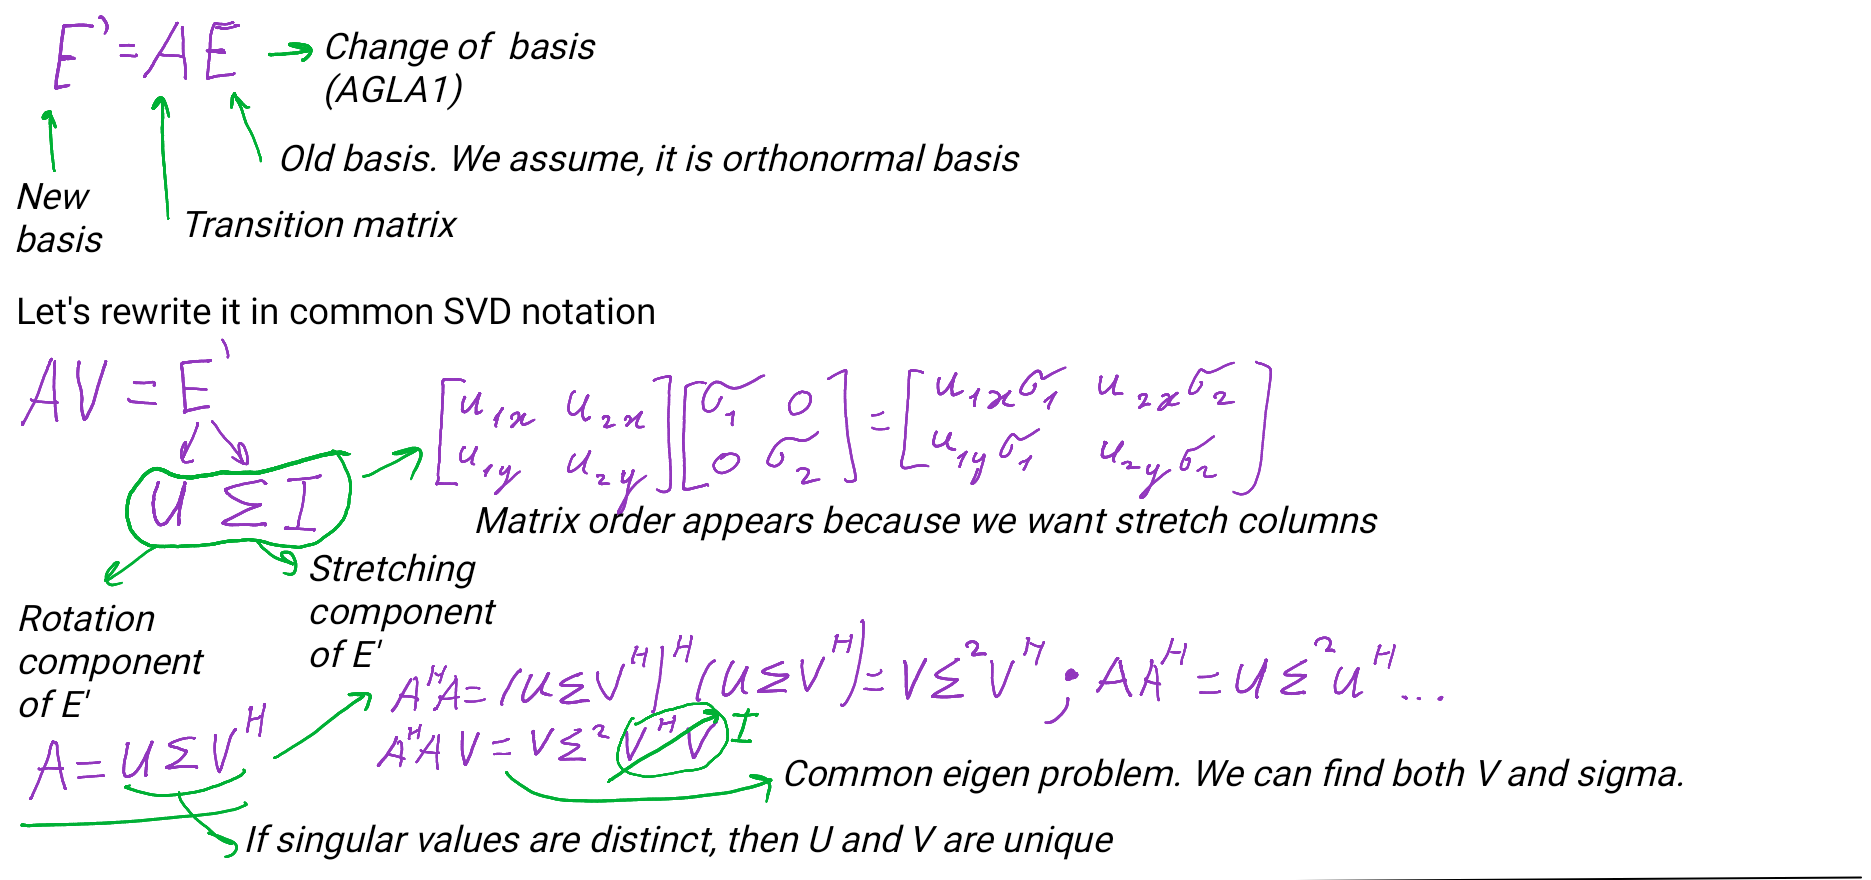
\includegraphics[height=6.5cm,width=1\textwidth,keepaspectratio]{svd_derive.png}
        % \caption{caption_name}
        \label{fig:svd_derive.png}
    \end{figure}
\end{frame}

\begin{frame}[t]{Singular Value Decomposition}
\framesubtitle{Geometrical explanation}
    \vspace{-0.5cm}
    \begin{figure}[H]
        \centering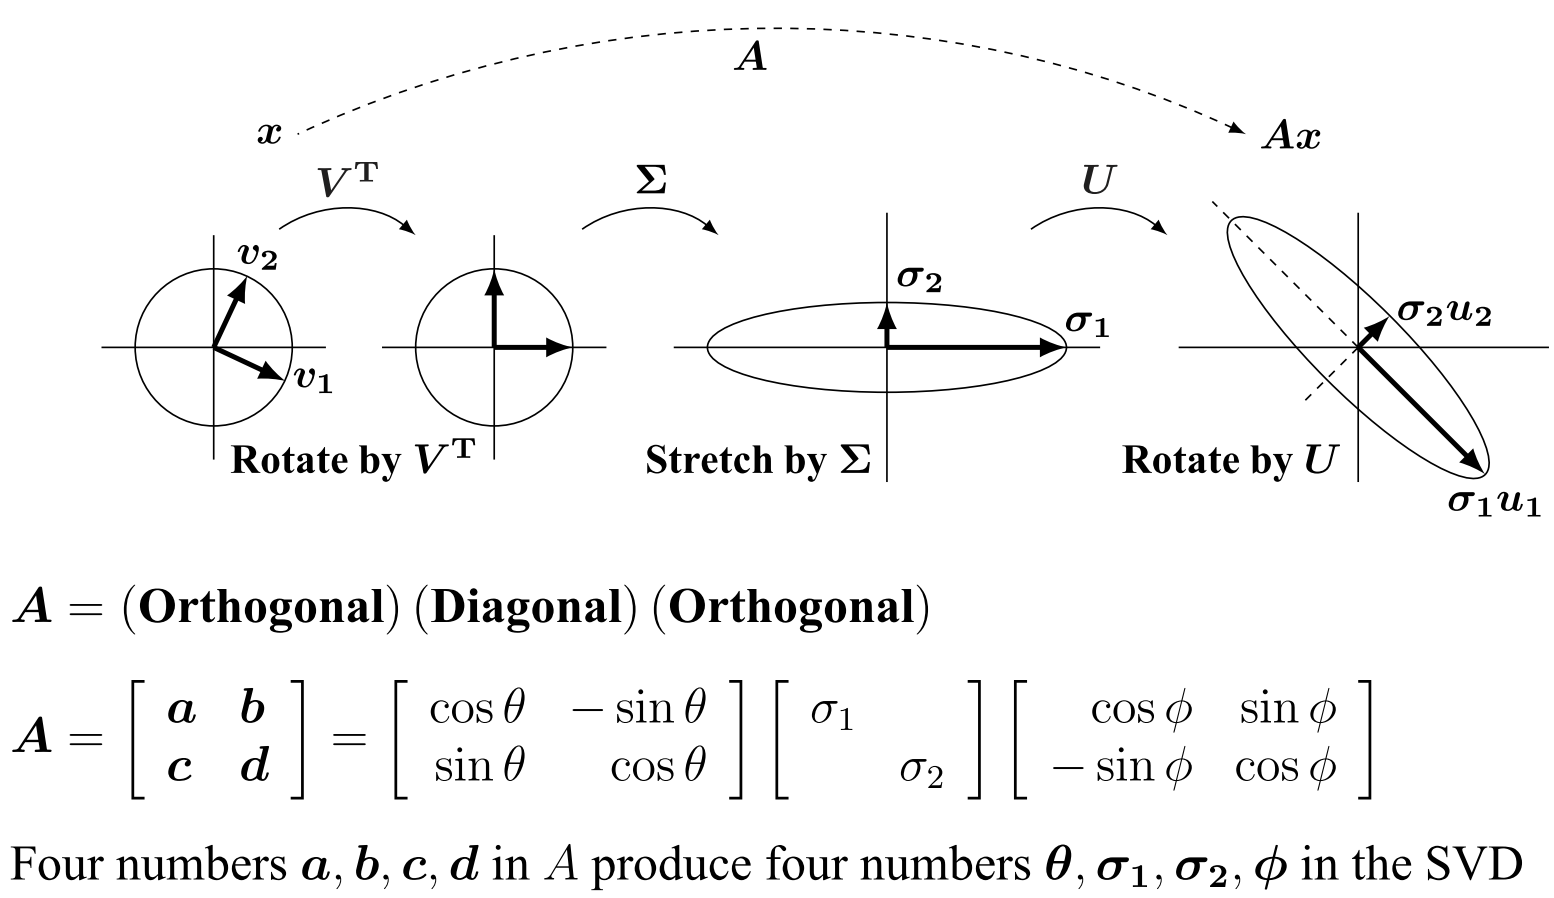
\includegraphics[height=6cm,width=1\textwidth,keepaspectratio]{svd_geometry.png}
        \label{fig:svd_geometry.png}
    \end{figure}
\end{frame}

\begin{frame}[t]{Singular Value Decomposition (SVD)}
\framesubtitle{How to calculate it (2 common ways)}
    \begin{block}{First approach}
        \begin{enumerate}
            \item Find eigenpairs for $A^TA$. Result is $\Sigma$ and $V$. ($A^TA=V\Sigma^{2}V^H$)
            \item Find $U$, using $\Sigma$ and $V$ ($AV\Sigma^{-1} = U$)
        \end{enumerate}
    \end{block}
    \begin{block}{Second approach}
        \begin{enumerate}
            \item Find eigenpairs for $A^TA$ and $AA^T$. ($A^TA=V\Sigma^{2}V^H$) ($AA^T=U\Sigma^{2}U^H$)
        \end{enumerate}
    \end{block}
\end{frame}

\begin{frame}[t]{Singular Value Decomposition (SVD)}
\framesubtitle{Obtain SVD for $A= \begin{bmatrix}
    3 & 2 & 2 \\
    2 & 3 & -2 
    \end{bmatrix}$, using second approach (\href{https://jonathan-hui.medium.com/machine-learning-singular-value-decomposition-svd-principal-component-analysis-pca-1d45e885e491}{task was taken})}
\vspace{-0.8cm}
    \begin{enumerate}
        \item Eigenpairs of $AA^T$.

        $AA^T=\begin{bmatrix}
        17 & 8\\ 
        8 & 17 
        \end{bmatrix}$. $\lambda_1 = 25$, $\lambda_2 = 9$. $x_{\lambda_1} = \begin{bmatrix}
        \frac{1}{\sqrt{2}}\\
        \frac{1}{\sqrt{2}}
        \end{bmatrix}$, $x_{\lambda_2} = \begin{bmatrix}
            \frac{1}{\sqrt{2}}\\
            -\frac{1}{\sqrt{2}}
            \end{bmatrix}$. $U = \begin{bmatrix}
                \frac{1}{\sqrt{2}} & \frac{1}{\sqrt{2}}\\ 
                \frac{1}{\sqrt{2}} &  -\frac{1}{\sqrt{2}}
            \end{bmatrix}$
        \item Eigenpairs of $A^TA$.
        
        $A^TA= \begin{bmatrix}
        13 & 12 & 2 \\
        12 & 13 & -2 \\ 
        2 & -2  & 8 
        \end{bmatrix}$. $\lambda_1 = 25$, $\lambda_2 = 9$, $\lambda_3 = 0$. $V = \begin{bmatrix}
            \frac{1}{\sqrt{2}} & \frac{1}{\sqrt{18}} & \frac{2}{3} \\
            \frac{1}{\sqrt{2}} & -\frac{1}{\sqrt{18}} & -\frac{2}{3}\\ 
            0 & \frac{4}{\sqrt{18}} & -\frac{1}{3}  
        \end{bmatrix}$
    \item Result. $A=U\Sigma V^T=\begin{bmatrix}
        \frac{1}{\sqrt{2}} & \frac{1}{\sqrt{2}}\\ 
        \frac{1}{\sqrt{2}} &  -\frac{1}{\sqrt{2}}
    \end{bmatrix}\begin{bmatrix}
    5 & 0 & 0 \\
    0 & 3 & 2 
    \end{bmatrix}\begin{bmatrix}
        \frac{1}{\sqrt{2}} & \frac{1}{\sqrt{2}} & 0 \\
        \frac{1}{\sqrt{18}} & -\frac{1}{\sqrt{18}} & \frac{4}{\sqrt{18}}\\ 
        \frac{2}{3} & -\frac{2}{3} & -\frac{1}{3}  
    \end{bmatrix}$
    \end{enumerate}
\end{frame}

\begin{frame}[t]{Task 1}
    \framesubtitle{}
    \vspace{-0.5cm}
    \begin{figure}[H]
        \centering
\includegraphics[height=3cm,width=1\textwidth,keepaspectratio]{1.png}
        % \caption{caption_name}
        \label{fig:1.png}
    \end{figure}
    \uncover<2->{
        \alert{\Large Answer}
        \begin{figure}[H]
            \centering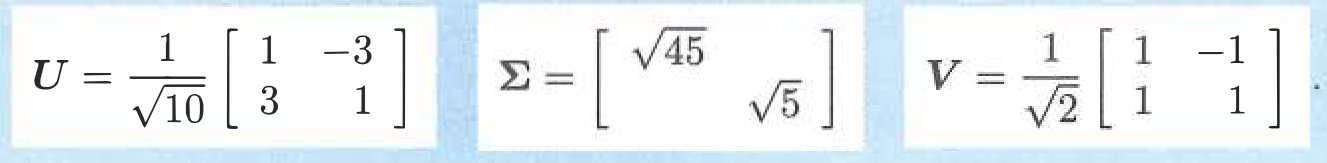
\includegraphics[height=3cm,width=1\textwidth,keepaspectratio]{1ans.png}
            % \caption{caption_name}
            \label{fig:1ans.png}
        \end{figure}
    }
\end{frame}

\begin{frame}[t]{It had to be $U$}  
    \framesubtitle{Video}
    \vspace{-0.6cm}
    \begin{figure}[H]
        \href{https://youtu.be/JEYLfIVvR9I}{
            \centering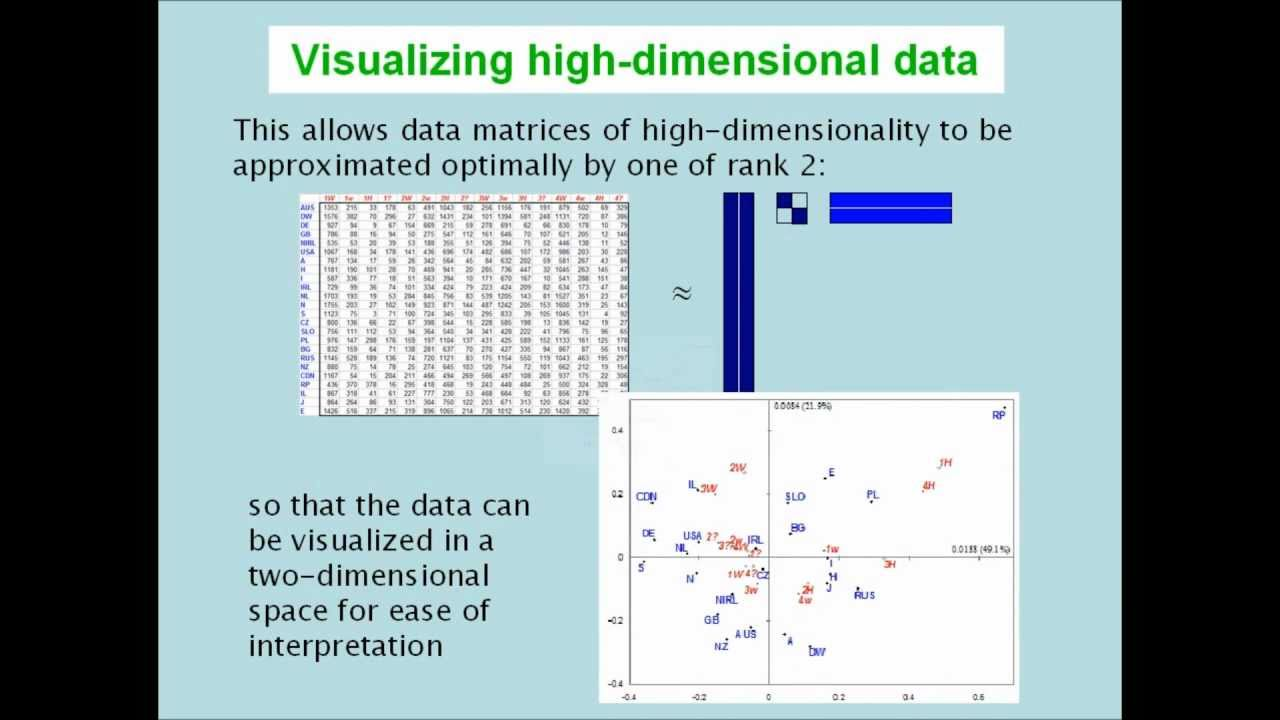
\includegraphics[height=6cm,width=1\textwidth,keepaspectratio]{svd_song.jpg}}
        % \caption{Click on a picture for a video}
        \label{fig:file_name}
    \end{figure}
\end{frame}

\begin{frame}[t]{Singular Value Decomposition (SVD)}
\framesubtitle{Properties}
    \LARGE 
    \begin{itemize}
        \item It is always possible to decompose a real matrix $A$ into SVD
        \item $U,\ \Sigma,\ V$ are unique
        \item $U,\ V$ -- column orthonormal
        \item By convention $\Sigma$ contains singular values in sorted order $\sigma_1 \geq \sigma_2 ...$ 
    \end{itemize}
\end{frame}

\begin{frame}[t]{Task 2}
    \framesubtitle{}    
    \only<1>{
    \vspace{-0.5cm}
    \begin{figure}[H]
        \centering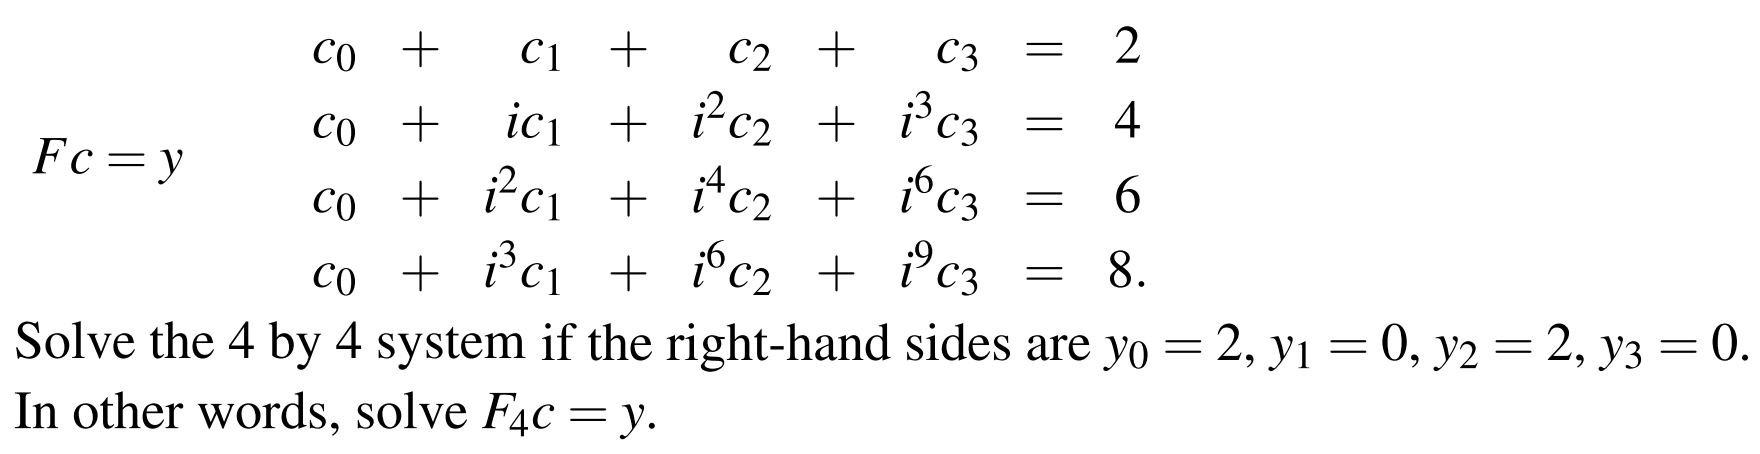
\includegraphics[height=3cm,width=1\textwidth,keepaspectratio]{2.png}
        % \caption{caption_name}
        \label{fig:2.png}
    \end{figure}
    }
    \only<2>{
        \alert{\Large Answer}
        \begin{figure}[H]
            \centering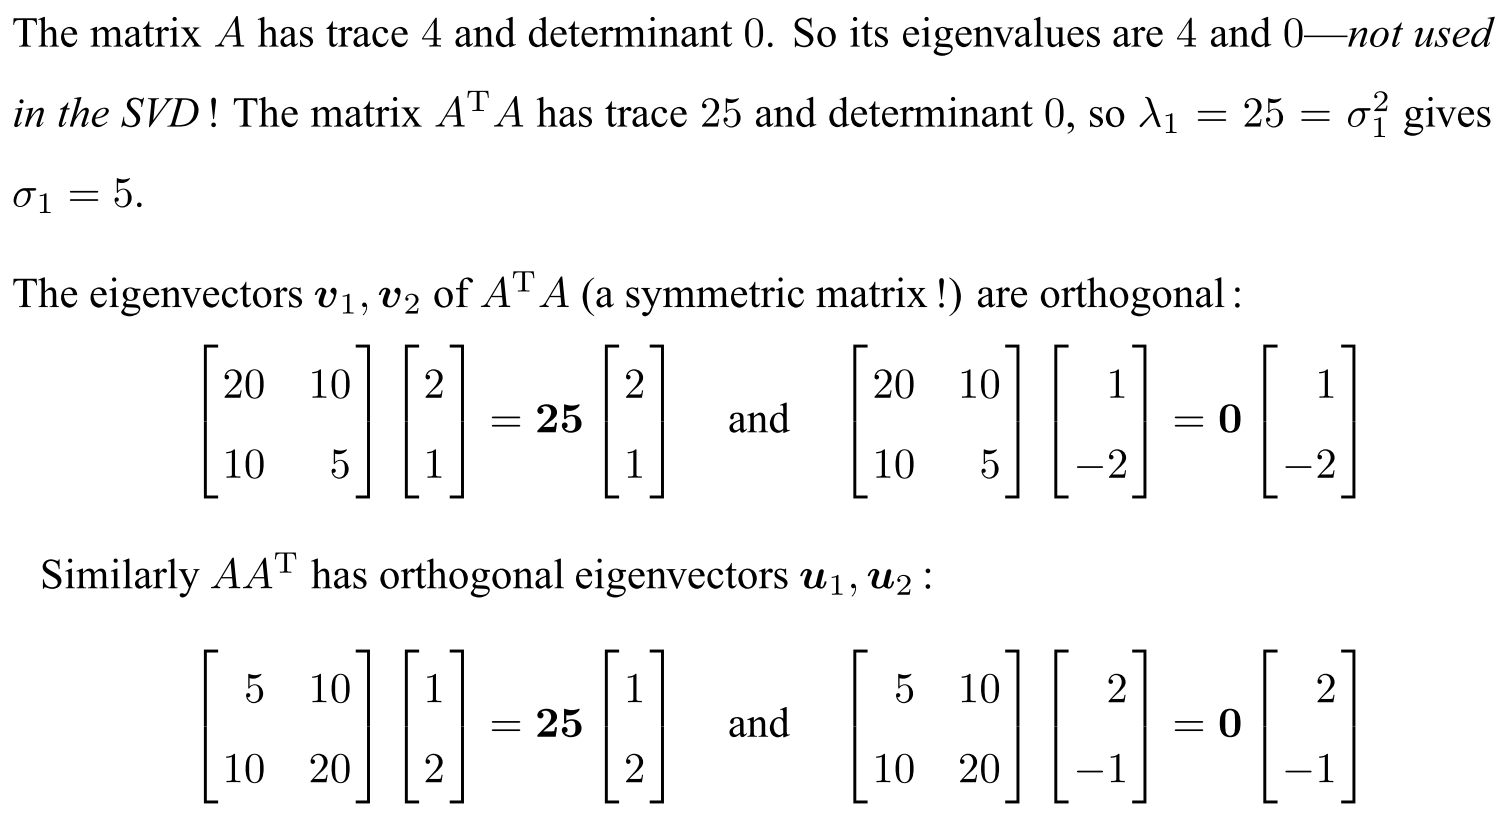
\includegraphics[height=5.5cm,width=1\textwidth,keepaspectratio]{2ans.png}
            % \caption{caption_name}
            \label{fig:2ans.png}
        \end{figure}
    }
\end{frame}

\usebackgroundtemplate{}
\setbeamercolor{background canvas}{bg=}
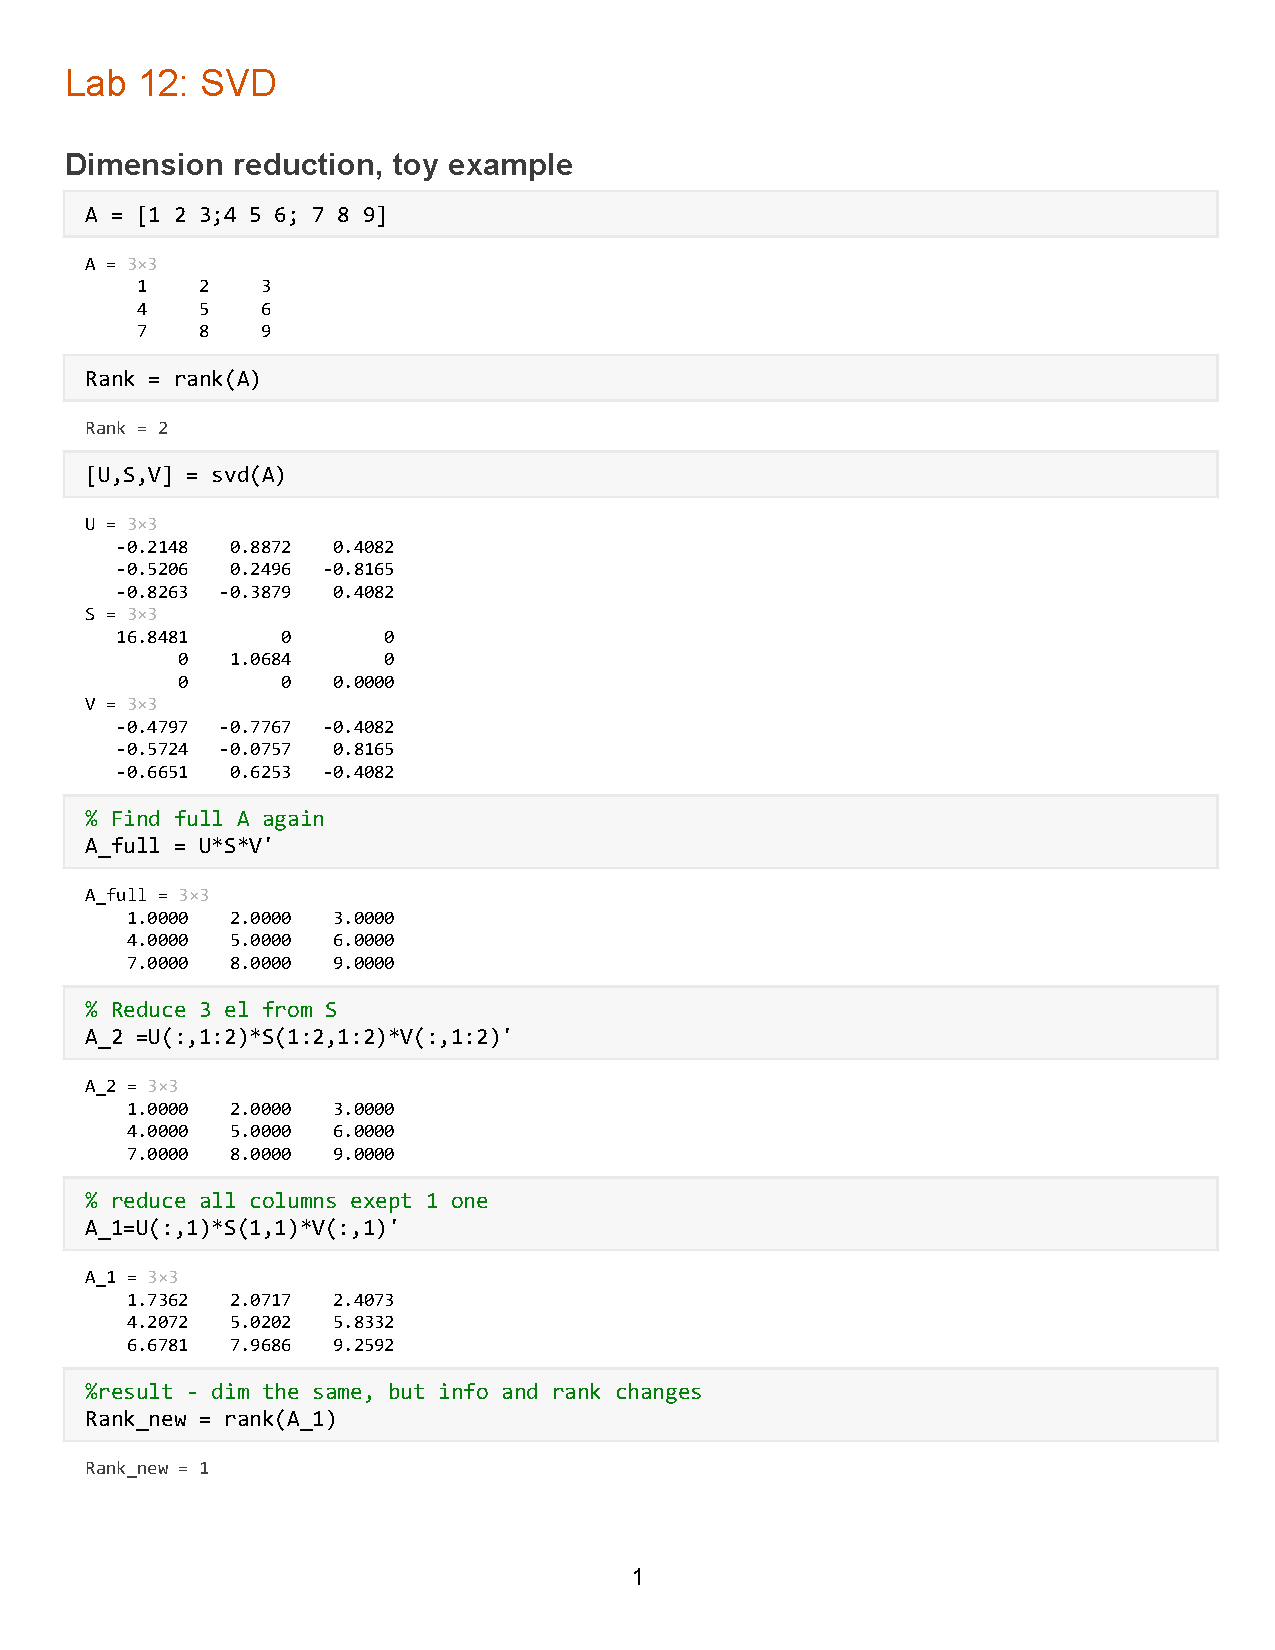
\includepdf[pages=-,fitpaper]{lab12_dimension_reduction.pdf}
\fbckg{fibeamer/figs/common.png}

\begin{frame}[t]{Task 3}
    \framesubtitle{}
    \vspace{-0.5cm}
    \begin{figure}[H]
        \centering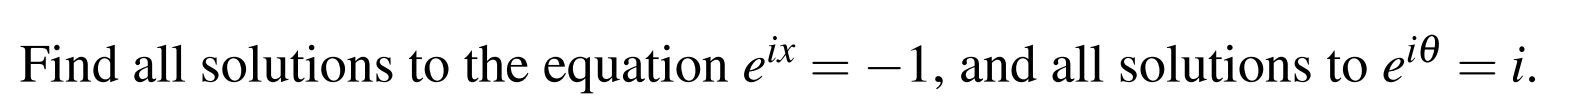
\includegraphics[height=3cm,width=1\textwidth,keepaspectratio]{3.png}
        % \caption{caption_name}
        \label{fig:3.png}
    \end{figure}
    \uncover<2->{
        \alert{\Large Answer}
        \begin{figure}[H]
            \centering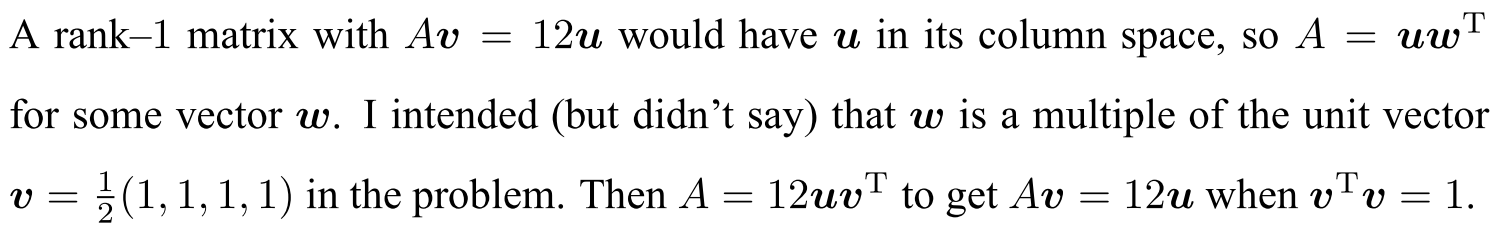
\includegraphics[height=3cm,width=1\textwidth,keepaspectratio]{3ans.png}
            % \caption{caption_name}
            \label{fig:3ans.png}
        \end{figure}
    }
\end{frame}


\begin{frame}[t]{Singular Value Decomposition (SVD)}
\framesubtitle{Where it can be used}
\Large
    \begin{itemize}
        \item For working with big datasets
        \item Image compression (on page \ref{image_compression})
        \item Pseudo-inverse (next slide)
        \item Least square (on page \ref{pdf_line_fitting})
        \item Principal Component Analysis (PCA) (\href{https://youtu.be/a9jdQGybYmE}{video})
        \item Eigenfaces algorithms (\href{https://youtu.be/_lY74pXWlS8}{video})
    \end{itemize}
\end{frame}

\usebackgroundtemplate{}
\setbeamercolor{background canvas}{bg=}
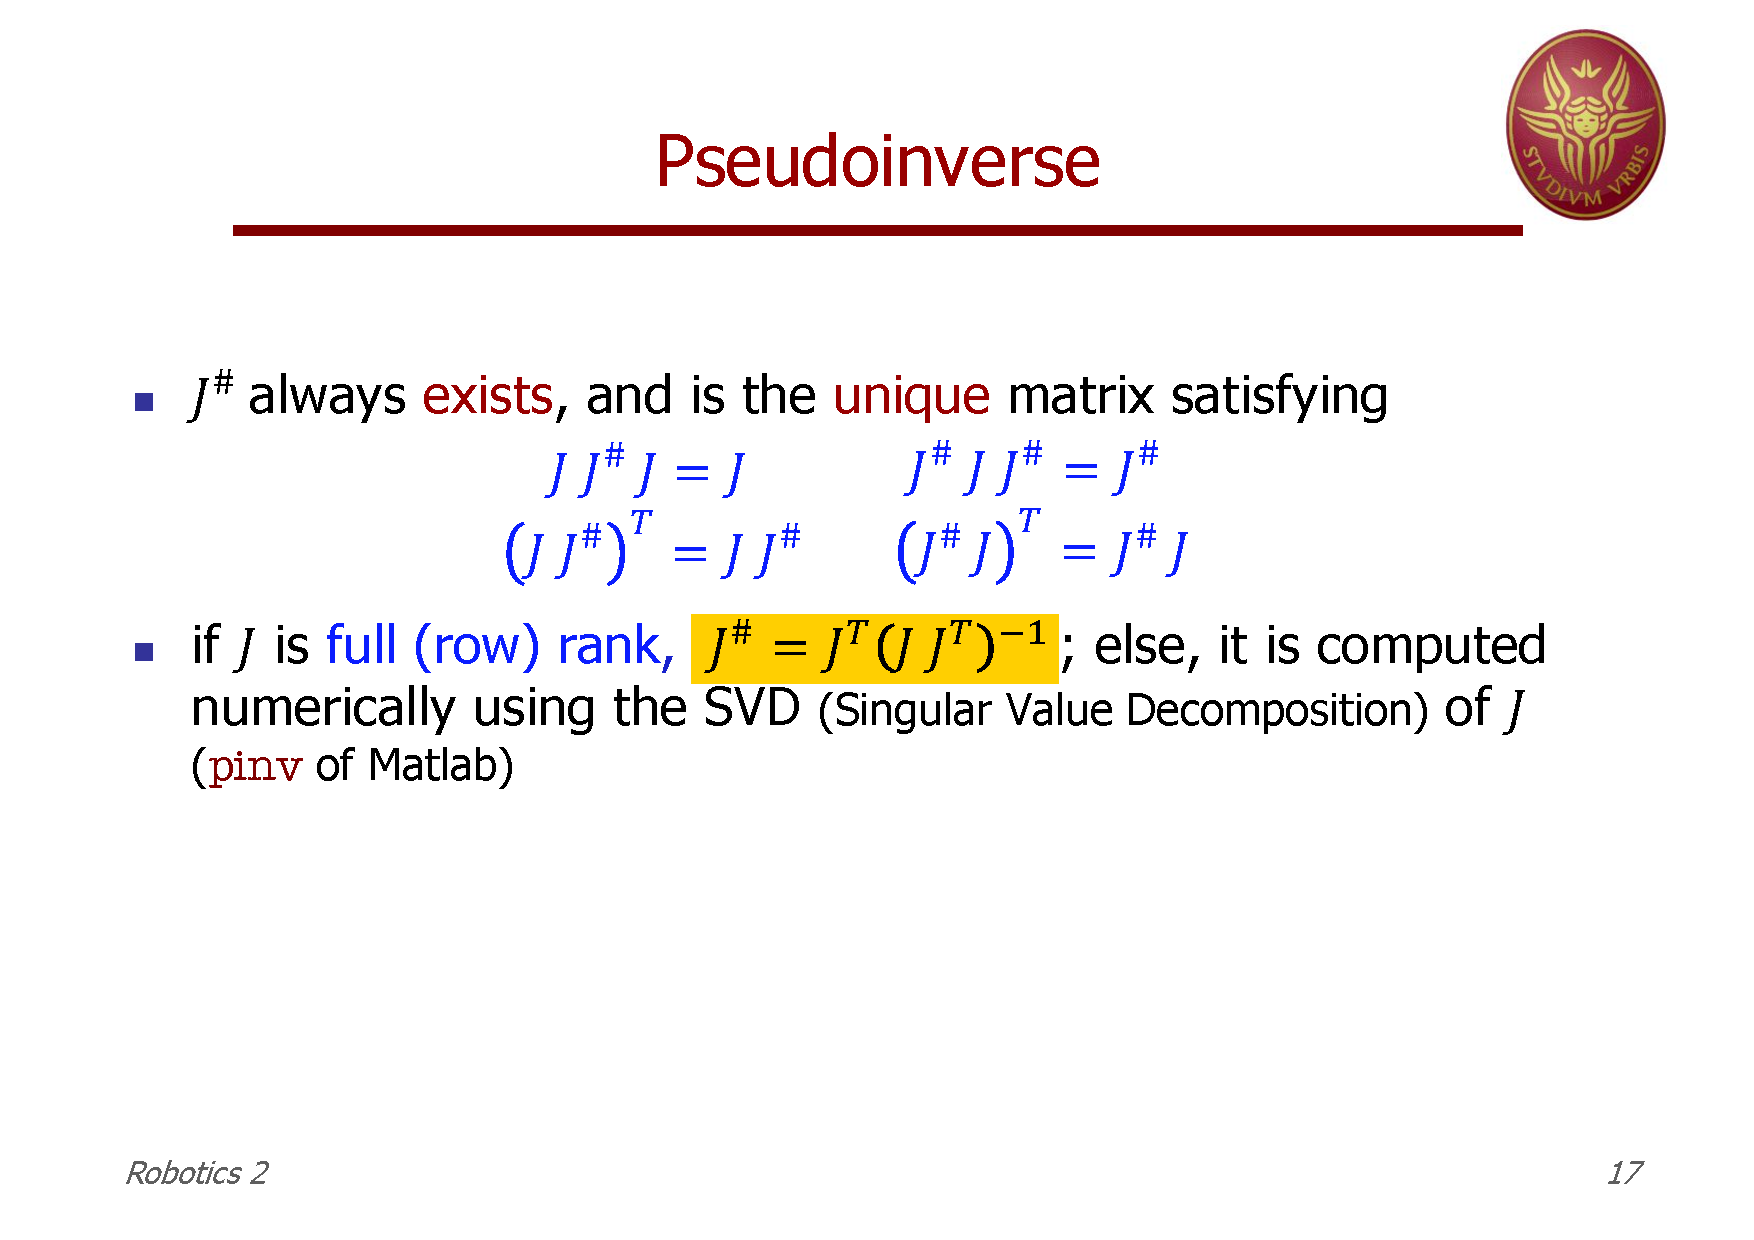
\includepdf[pages=-]{pseudoinverse.pdf}
\fbckg{fibeamer/figs/common.png}

\note{Сказать, что псевдоинверсия может обозначаться как решетка, так и плюсик ($J^+ = J^{\#}=J^{\dagger}$)}

\begin{frame}[t]{Task 4}
    \framesubtitle{}
    \vspace{-0.5cm}
    \begin{figure}[H]
        \centering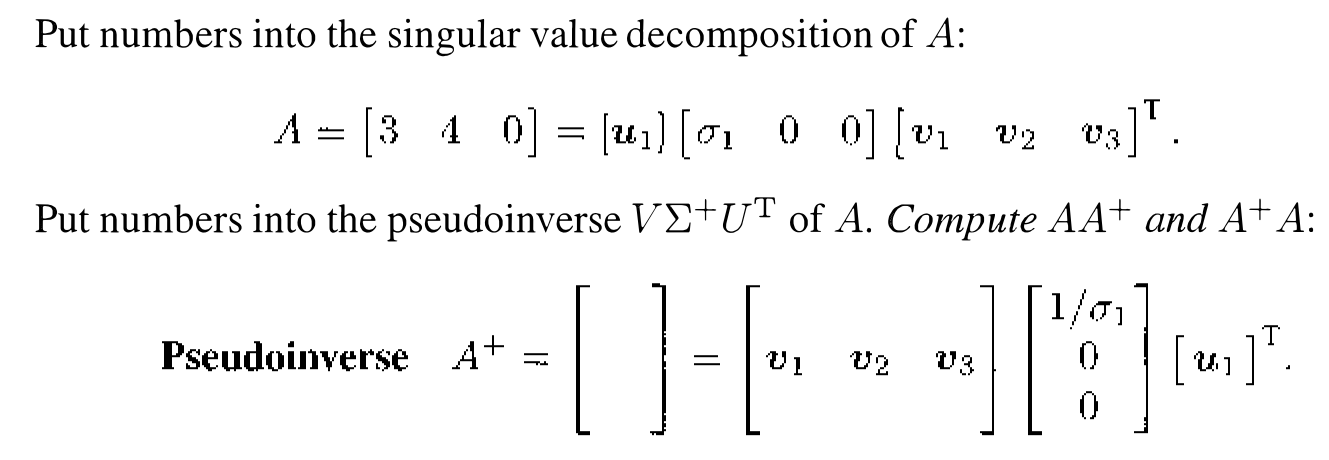
\includegraphics[height=3cm,width=1\textwidth,keepaspectratio]{4.png}
        % \caption{caption_name}
        \label{fig:4.png}
    \end{figure}
    \uncover<2->{
        \alert{\Large Answer}
        \begin{figure}[H]
            \centering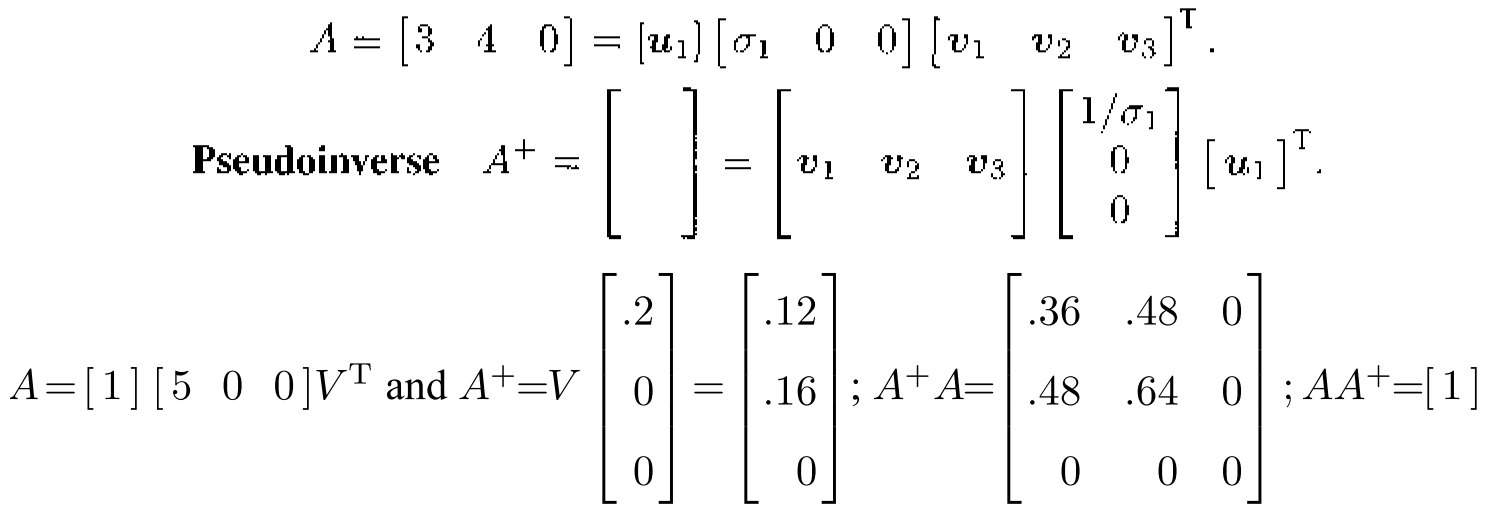
\includegraphics[height=3cm,width=1\textwidth,keepaspectratio]{4ans.png}
            % \caption{caption_name}
            \label{fig:4ans.png}
        \end{figure}
    }
\end{frame}

\begin{frame}[t]{SVD Applications}
    \framesubtitle{Video: Users-to-Movies}
    \vspace{-0.6cm}
    \begin{figure}[H]
        \href{https://youtu.be/P5mlg91as1c?t=466}{
            \centering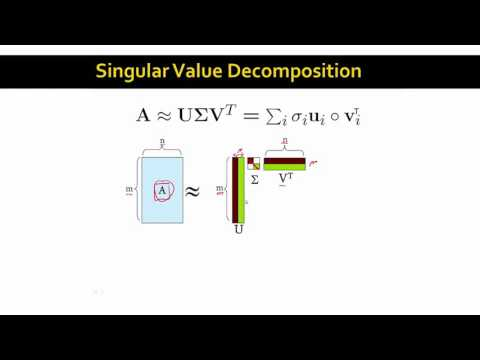
\includegraphics[height=6cm,width=1\textwidth,keepaspectratio]{svd_example_stanford.jpg}}
        % \caption{Click on a picture for a video}
        \label{fig:svd_example_stanford.jpg}
    \end{figure}
\end{frame}

\begin{frame}[t]{Task 5}
    \framesubtitle{}
    \only<1>{
    \vspace{-0.5cm}
    \begin{figure}[H]
        \centering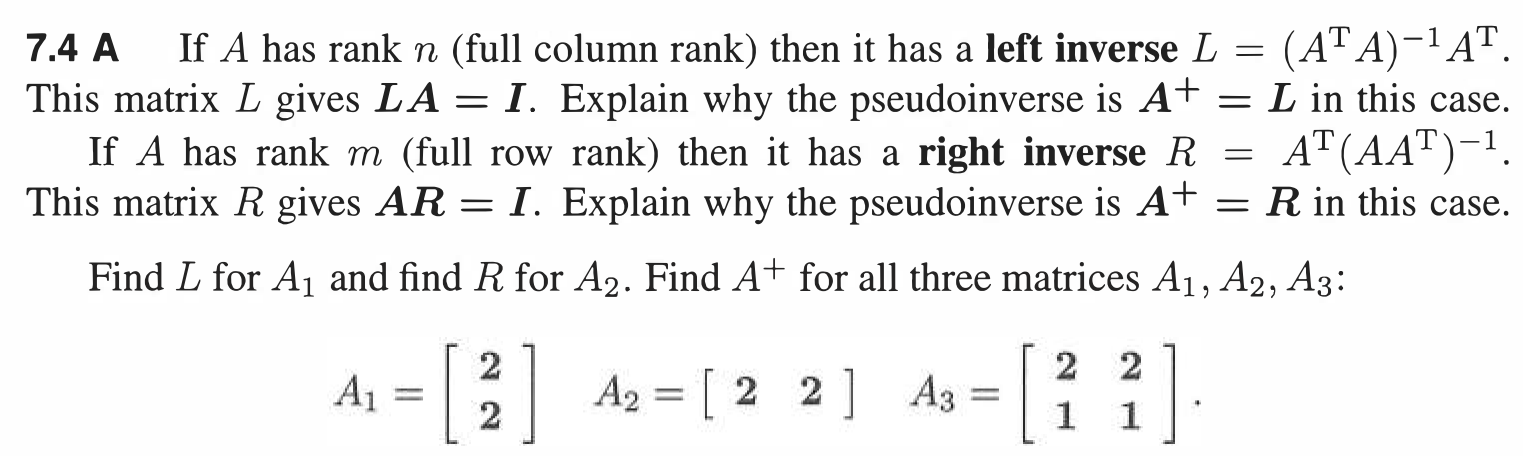
\includegraphics[height=3cm,width=1\textwidth,keepaspectratio]{5.png}
        % \caption{caption_name}
        \label{fig:5.png}
    \end{figure} }
    \only<2>{
        \alert{\Large Answer}
        \begin{figure}[H]
            \centering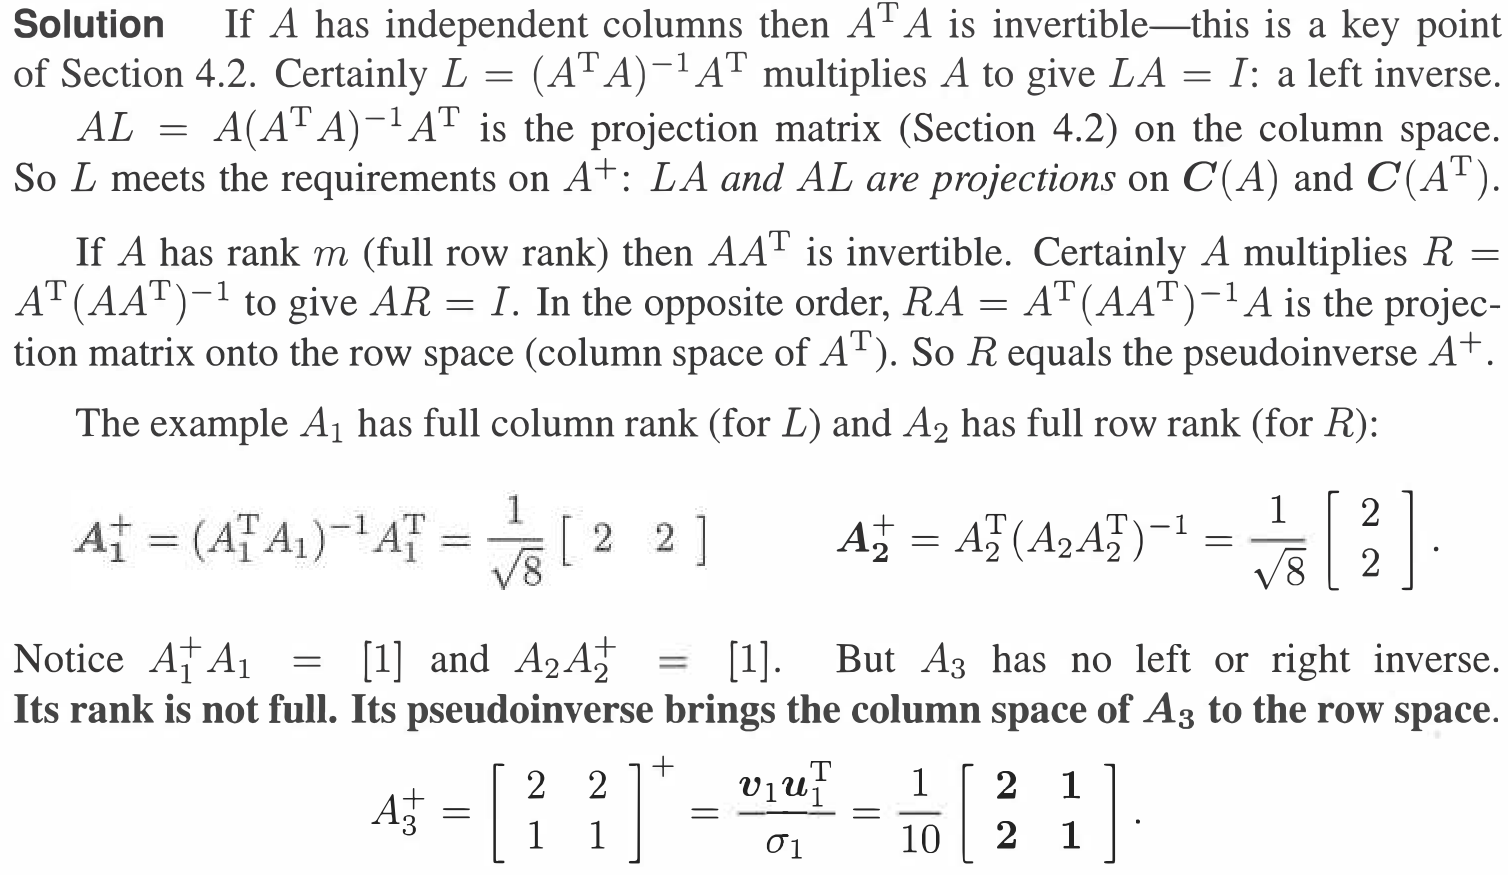
\includegraphics[height=5.5cm,width=1\textwidth,keepaspectratio]{5ans.png}
            % \caption{caption_name}
            \label{fig:5ans.png}
        \end{figure}
    }
\end{frame}

\begin{frame}[t, label=image_compression]{SVD Applications}
\framesubtitle{Image compression}
\begin{columns}[T,onlytextwidth]
    \begin{column}{0.39\textwidth}
        \textit{\underline{Task:}} We want to compress our image for reducing the size.

\textit{\underline{Solution:}} We can represent our picture as a matrix. 

Next step is using SVD for reducing matrix rank.

Code on page \ref{pdf_image_compressing}

    \end{column}
    \begin{column}{0.59\textwidth}
        \vspace{-1cm}
        \begin{figure}[H]
            \centering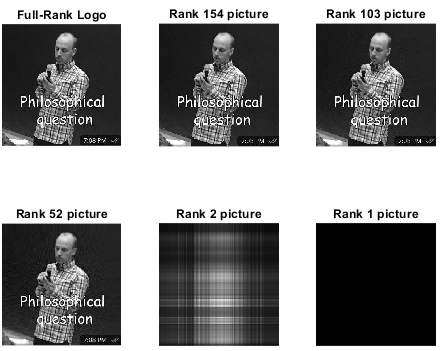
\includegraphics[height=6cm,width=1\textwidth,keepaspectratio]{image_proc.png}
            \label{fig:image_proc.png}
        \end{figure}
    \end{column}
\end{columns}
    
\end{frame}

\begin{frame}[t]{Task 6}
    \framesubtitle{}
    \vspace{-0.5cm}
    \begin{figure}[H]
        \centering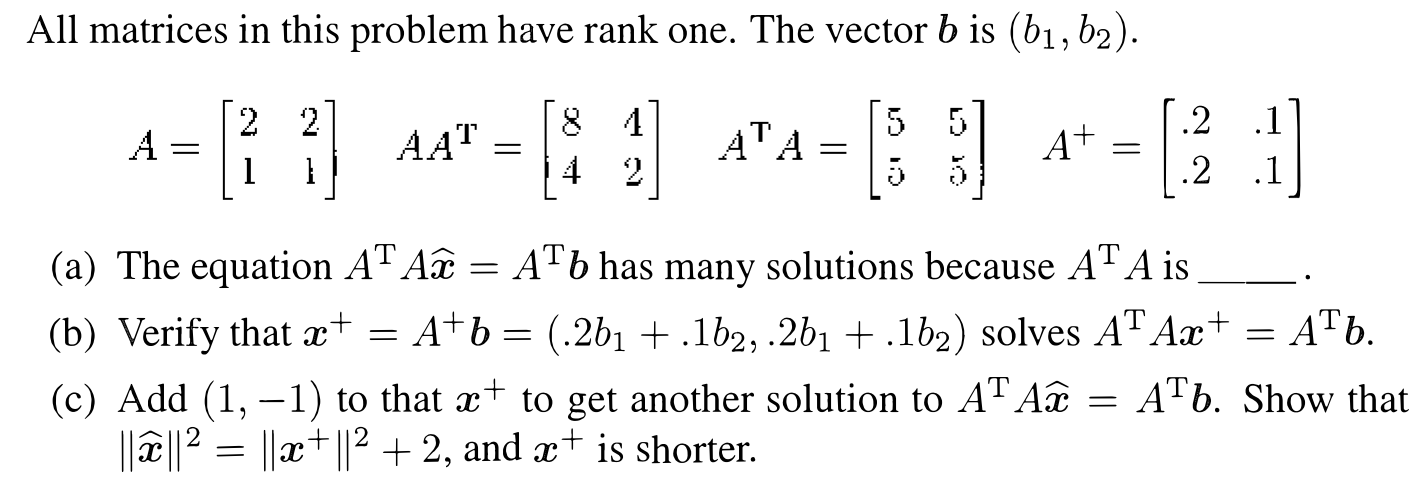
\includegraphics[height=3cm,width=1\textwidth,keepaspectratio]{6.png}
        % \caption{caption_name}
        \label{fig:6.png}
    \end{figure}
    \uncover<2->{
        \vspace{-0.5cm}
        \alert{\Large Answer}
        \begin{figure}[H]
            \centering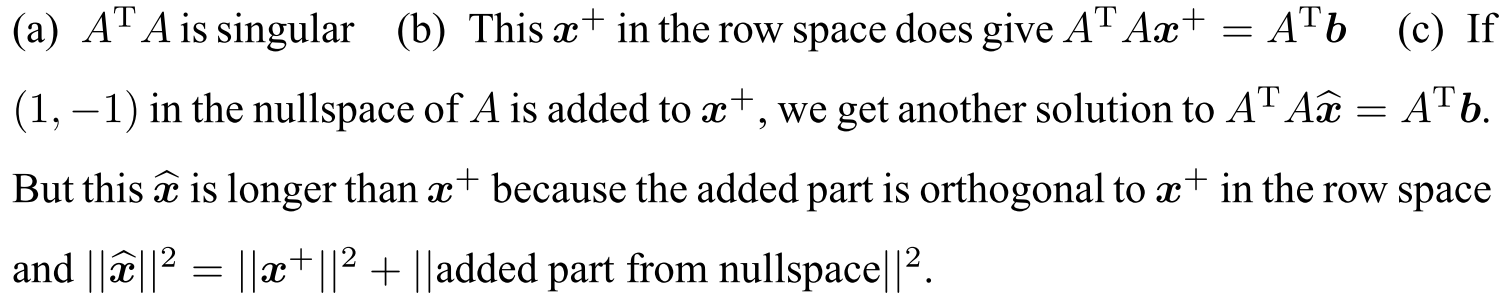
\includegraphics[height=2.5cm,width=1\textwidth,keepaspectratio]{6ans.png}
            % \caption{caption_name}
            \label{fig:6ans.png}
        \end{figure}
    }
\end{frame}

\begin{frame}[t]{Reference material}
    \framesubtitle{}
    \large
    \begin{itemize}
        \item \href{https://www.youtube.com/watch?v=TSdXJw83kyA}{Lecture 28: Similar Matrices and Jordan Form.}
        \item \href{https://www.youtube.com/watch?v=Nx0lRBaXoz4&list=PL49CF3715CB9EF31D&index=30}{Lecture 29: Singular Value Decomposition}
        \item \href{https://www.youtube.com/watch?v=Go2aLo7ZOlU&list=PL49CF3715CB9EF31D&index=34}{Lecture 33: Left and Right Inverses; Pseudoinverse}
        \item \href{https://www.youtube.com/watch?v=rYz83XPxiZo&list=PLUl4u3cNGP63oMNUHXqIUcrkS2PivhN3k&index=8}{6. Singular Value Decomposition (SVD)}
        \item \textit{"Introduction to Linear Algebra", pdf pages 375--411 }\\  7 Singular Value Decomposition (SVD)
        \item \textit{"Linear Algebra and Applications", pdf pages 335--345 }\\ 5.6 Similarity Transformations
        \item \textit{"Linear Algebra and Applications", pdf pages 377--386 }\\ 6.3 Singular Value Decomposition
    \end{itemize}
\end{frame}

\fbckg{fibeamer/figs/last_page.png}
\frame[plain]{}
\fbckg{fibeamer/figs/common.png}

\begin{frame}[label=pdf_line_fitting]{Appendix: Line fitting pdf}
    \LARGE
    \centering
    Next Slide
\end{frame}

\usebackgroundtemplate{}
\setbeamercolor{background canvas}{bg=}
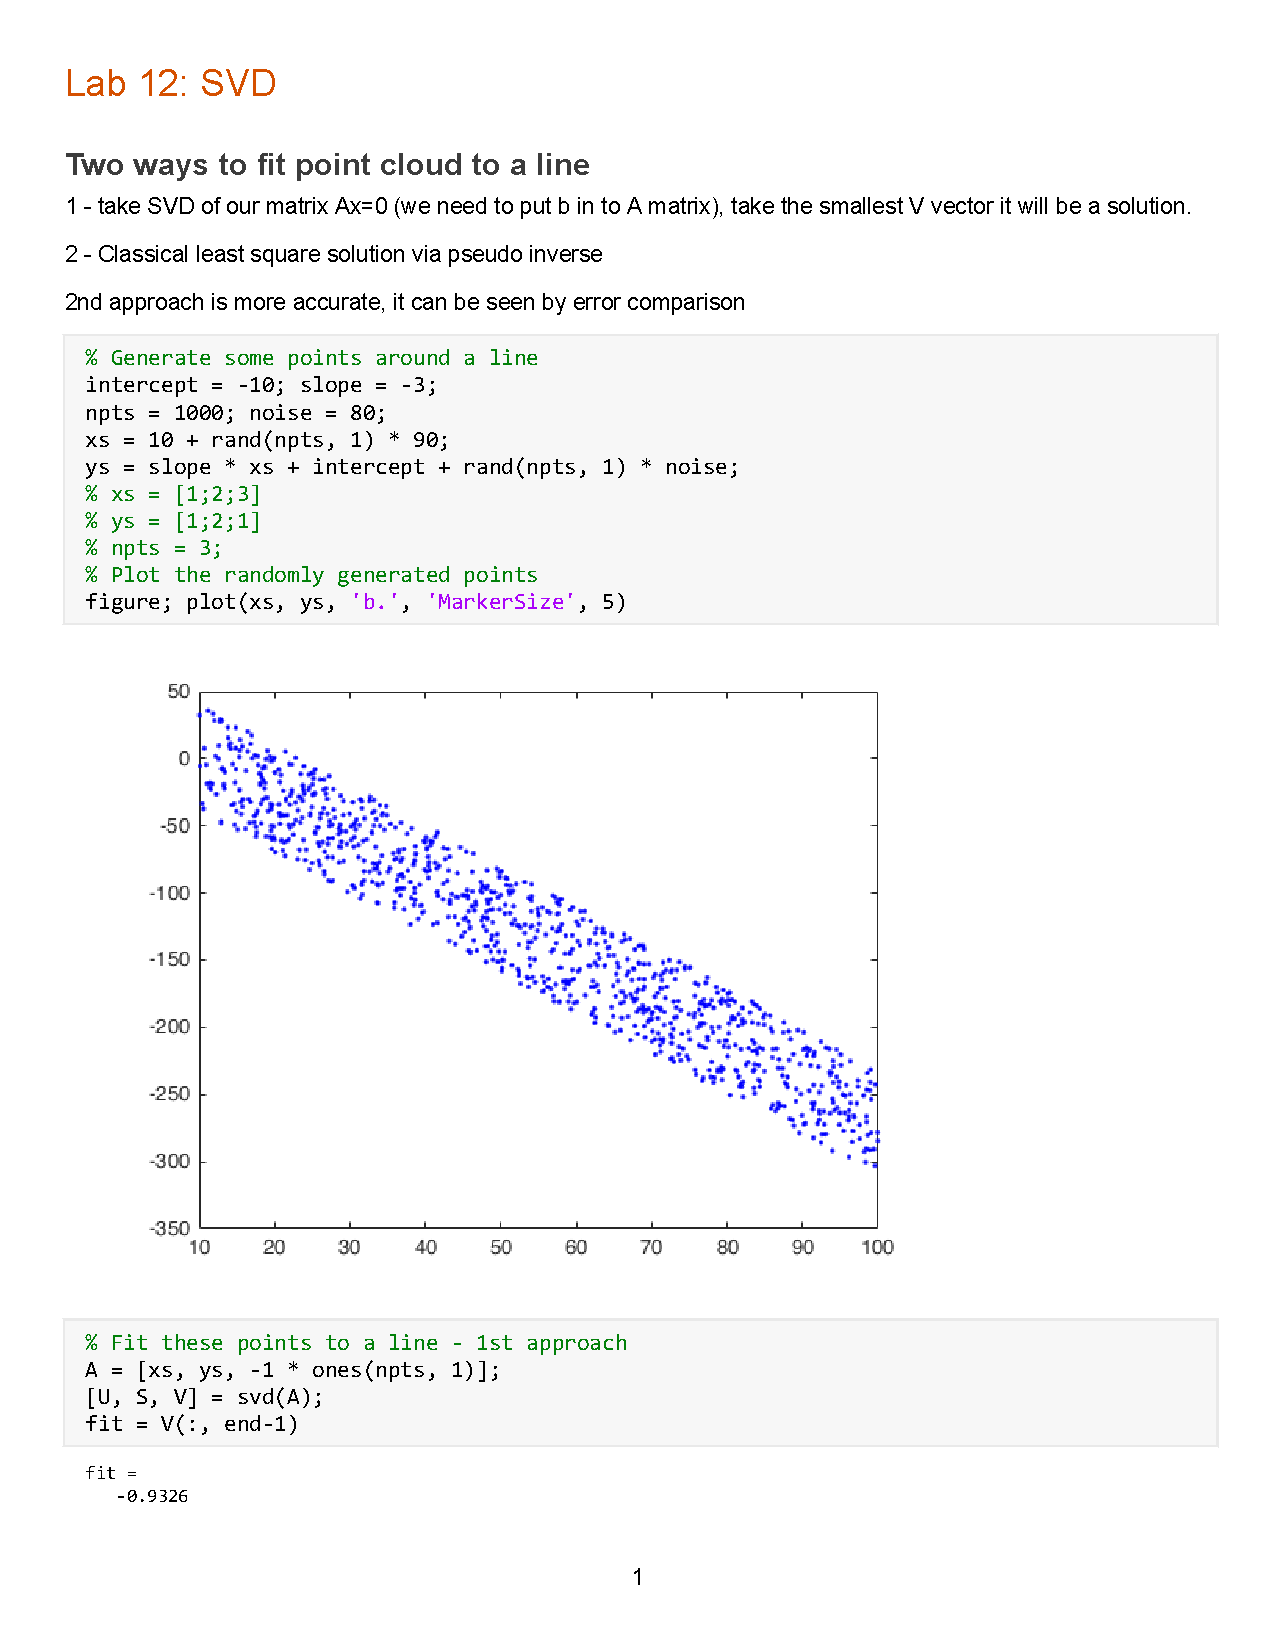
\includepdf[pages=-,fitpaper]{lab12_fit_line.pdf}
\fbckg{fibeamer/figs/common.png}

\begin{frame}[label=pdf_image_compressing]{Appendix: Image compressing pdf}
\framesubtitle{}
\LARGE
\centering
Next Slide
\end{frame}

\usebackgroundtemplate{}
\setbeamercolor{background canvas}{bg=}
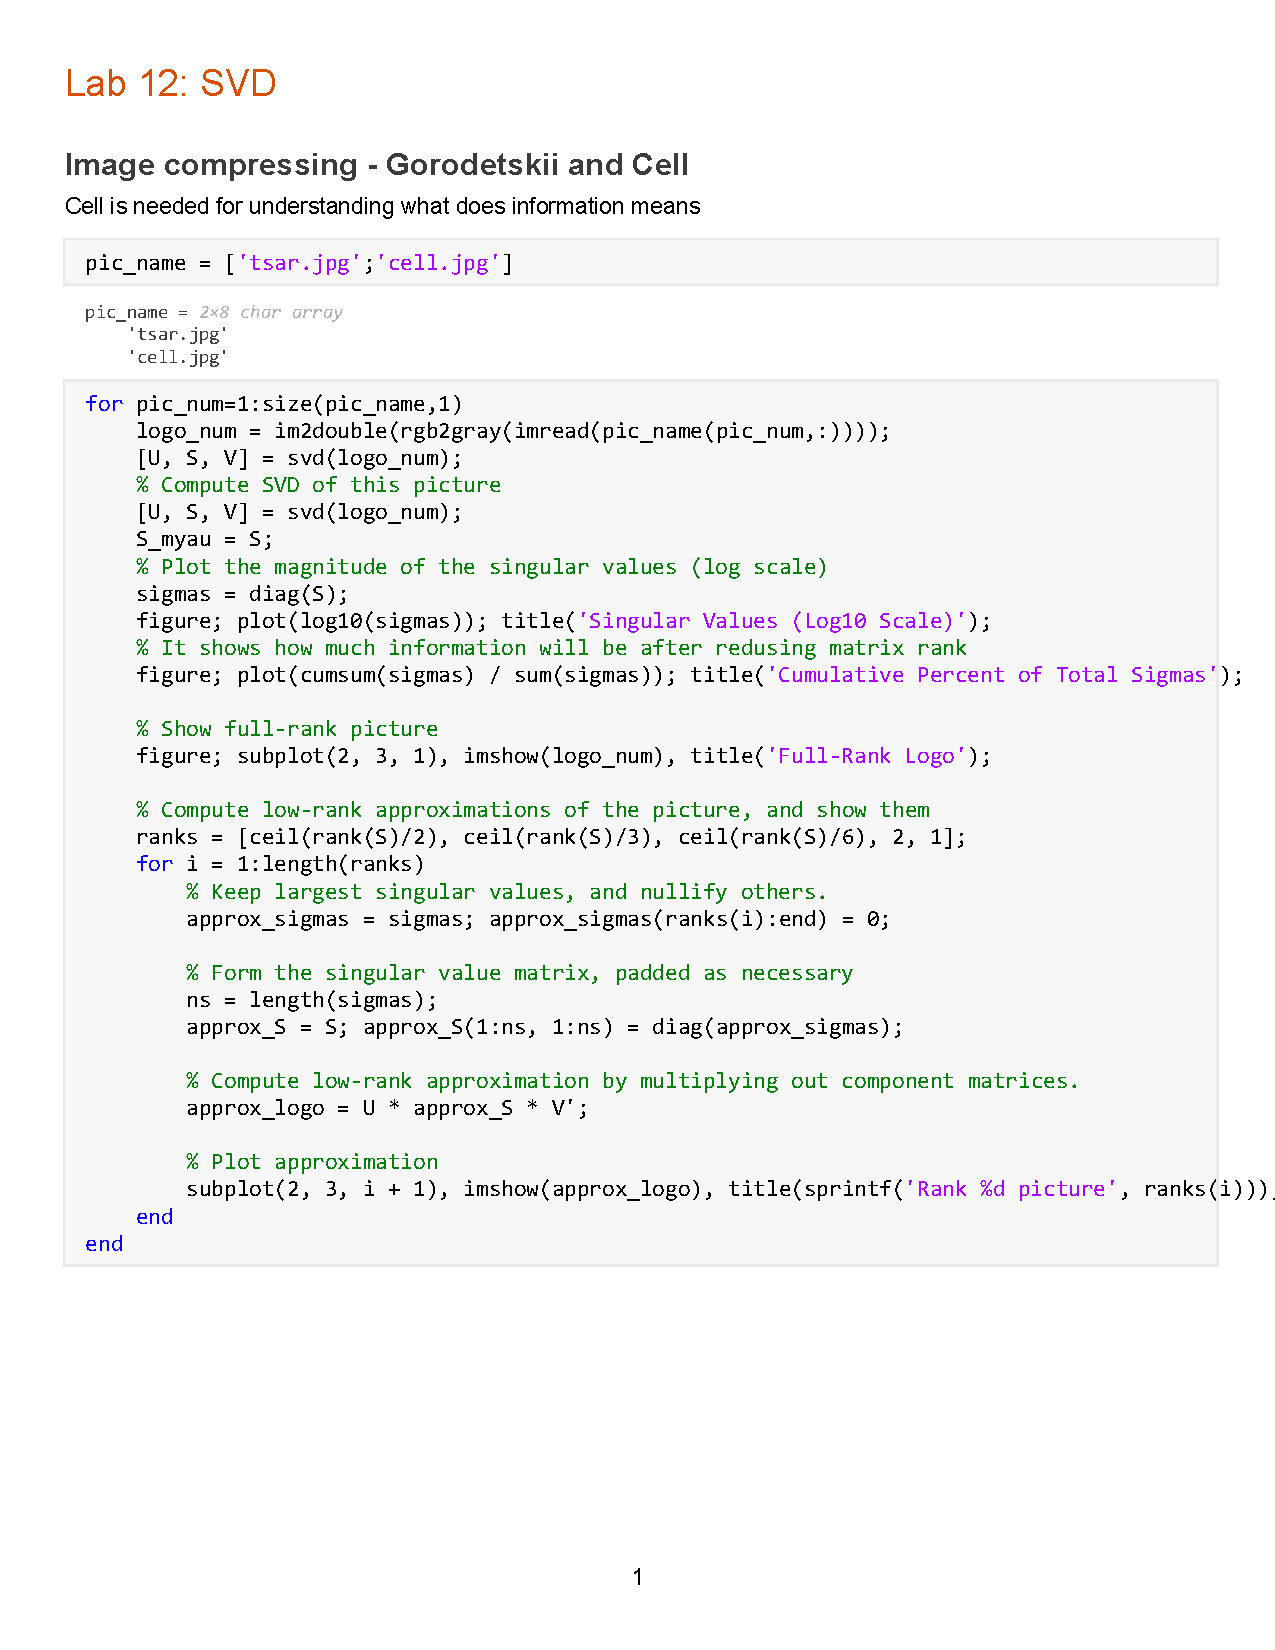
\includepdf[pages=-,fitpaper]{lab12_image_compressing.pdf}
\fbckg{fibeamer/figs/common.png}

\end{document}